%Anna

% Domain layer 
% Data layer (firebase)
% tactics
%  - interfaces and listeners (dependecy injection) (composite pattern?)
%  - activity recognition vs significant
%  - No Location - new model for calculations
% choice of tecnhologies and sensors

\section{Application Architecture}



\section{Continuous Sensing Architecture}

The continuous sensing in this application is formed from the notions of:
\begin{itemize}
    \item Geofence 
    \item Location 
    \item Activity Recognition
\end{itemize}

When the user creates or applies to a bikebus two Geofences are created for the start and end destination on the route. When the user is within the one of the Geofences, the Geofence fires an event which either initiates or stops the data collection.
Concretely the application holds a SensorDataController, which controls the flow of sensor data. 
\begin{enumerate}
    \item Creating two Geofence pending intents from the GoogleGeofence class
    \item The GeofenceIntentService class receives a GoogleGeofenceEvent object when a Geofence is triggered
    \item Based on the information from the Geofence event the GeofenceIntentService sends a status and result value back to the SensorDataController through a BroadcastReceiver
    \item The SensorDataController either stops the activity recognition or creates pending intents at a given sample rate from the GoogleActivityRecognition class
    \item Each time the ActivityRecognizeService class receives an intent with a ActivityRecognitionResult object the intent service broadcasts the results back to the SensorDataController
    \item Based on the activity has the value "ON\_BICYCLE" the SensorDataController will retrieve the current location of the user and store all locations for data processing
\end{enumerate}

\begin{figure}[H]
\centering
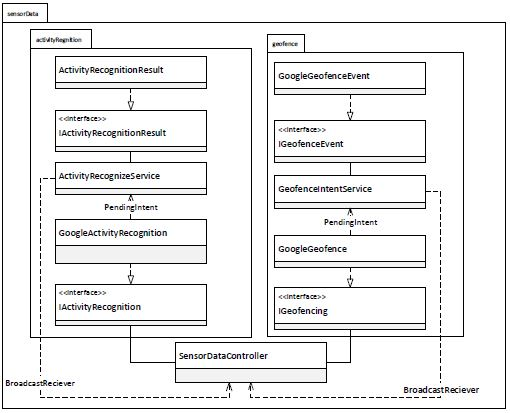
\includegraphics[scale=0.8]{Graphics/Images/Module_View_SensorData.jpg}
\caption{Module view of sensorData package}
\label{fig:Module_View_Sensor_Data}
\end{figure}
In figure \ref{fig:Module_View_Sensor_Data} a module view has been created based on the continuous data collection description. 

In Android there is typically two methods to apply when wanting to create background processes:
\begin{itemize}
    \item IntentService
    \item AsyncTask
\end{itemize}

The IntentService is a method used for long-term running background processes that is not dependent on the Activity. The AsyncTask is oppositely a method that only exists in the Activity's lifecycle, because it needs to return the value directly to the Activity. Therefore the AsyncTask cannot continue to run outside the application, and is more suited for short-term running background processes which are dependent on the Activity. 
\footnote{\url{https://github.com/codepath/android_guides/wiki/Starting-Background-Services}}

\section{Domain layer}

The domain layer of the application contains three central classes and two enum classes. In figure \ref{fig:domain_layer} below a class diagram have been constructed of those classes. 

\begin{figure}[H]
    \centering
    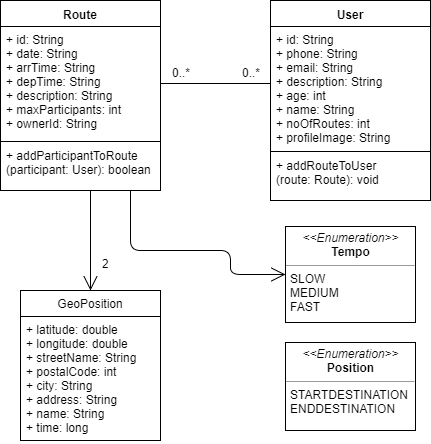
\includegraphics[scale=0.5]{Graphics/Images/domain_class_diagram.png}
    \caption{Class Diagram of Domain Layer}
    \label{fig:domain_layer}
\end{figure}

It can be seen that the "Route" and "User" classes have a tight relationship. Each route has a list of users as participants (excluding the owner), and each user has a list of created or applied to routes. This is a independent relationship, because a route can exist without any participants, and a user can exist without any routes created or applied to.

A "Route" contains two "GeoPosition" references as start destination and end destination.
The "GeoPosition" class can be instantiated by only latitude and longitude but also by the coordinates and an address. The address can be either a streetname, city and postal code, or if it is a public place i.e. "Odense Zoo" it can be name and and an address. The get methods will automatically return the correct data regardless of the construction, including potientially calculating the address from only coordinates using the static "AddressService" class which uses the "Geocoder" library.

The "Tempo" enum class is used to denote the tempo of a given route. Currently the user chooses the tempo subjectively when creating a route, but an idea for future work is to calculate the tempo automatically based on the distance and the guiding duration.

The "Position" enum class is currently only used when handling geo-fences in the data collection to determine whether the activated geo-fence is a start or end destiantion.

\section{Graphical User Interface}
The graphical design of this application is strongly inspired from another app called "GoMore", which has the concept of coordinating carpools. The "GoMore" concept reminds a lot about the "BikeBus" concept, because both apps coordinates for friends and strangers to ride with each other. The main differences between the two concepts are that "BikeBus" coordinates free bicycle rides and paid "GoMore" coordinates Car rides.

The graphical user interface of the application is developed using the Android API, which connects each view with an activity. In figure \ref{fig:activities} below a diagram shows the connections between each activities, where the dotted line represents the navigation between views using the "startActivity" method, and the other arrows follows UML by showing inheritance and association between the classes.   

\begin{figure}[H]
    \centering
    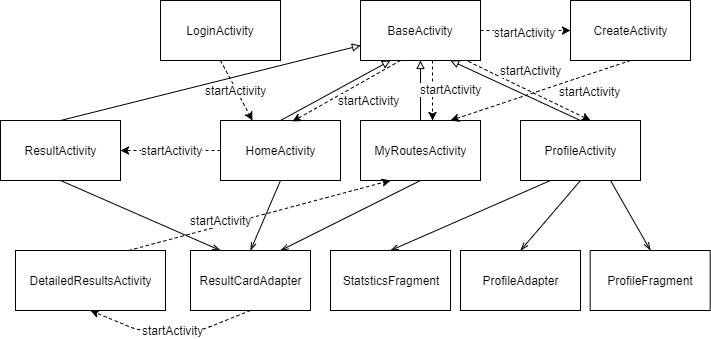
\includegraphics[scale=0.5]{Graphics/Images/Activity_Diagram.png}
    \caption{Diagram of activities}
    \label{fig:activities}
\end{figure}

As it can been seen in the figure, four activities inherits from the "BaseActivity" class, which sets the bottom navigation bar and the floating create button. The create button is though removed from the "ProfileActivity". 
This structure collects the base functionalities for some of the activities to make it easily modifiable.
Beside from the activity classes, the diagram also contains fragment and adapter classes. The two fragment classes "ProfileFragment" and "StatisticsFragment" coexists with the "ProfileAdapter" class to create a tab view, where the user can switch between profile and statistics information in the same activity. The "ResultCardAdapter" is used by three different activities because it implements a generic way of presenting a list of information viewed as "cards" in the material design. These cards are used in the "HomeActivity" as a list of recent routes, the "ResultActivity" as a search result list of routes, and the "MyRoutesActivity" as a list of routes created of applied to by the user. Again this adapter work generically, making it possible for multiple activities to use the functionality in different cases easily.

\subsection{Data Layer}

In order to create and search through routes across multiple devices and users, a database must be created to store all route and user information.
We have chosen to create the database in Firebase, which is a real-time document database hosted by Google. As Firebase is hosted by Google online it is therefore server-less and easy to setup and manage. On the other the application cannot retrieve data offline, and it becomes quite inconvenient to create a manual caching layer. Firebase is a NoSQL database, which means all querying has to be done manually. Firebase only returns a "snapshot" of the data at a given place in the database, and that should be information enough making querying disposable. This simple database structure becomes very scalable and performs very well for retrieval, which typically is the main requirements for real time mobile applications.

Firebase stores JSON trees of strings, which can easily be serialized into objects in Java. Best-practices of these JSON trees are to make the tree as flat as possible with references to objects. If the JSON tree is too deep and contains multiple layer of nested objects, the data snapshot retrieved for the application becomes very large and possibly very extravagant. Therefore it is more efficient to store a list of each object type containing meta data and a reference to possibly nested objects to be looked up in another data snapshot.

% Why store google account data when already logging in with google?
Currently our database looks as the following:
\begin{figure}[!htb]
    \centering
    \begin{minipage}{.5\textwidth}
        \centering
        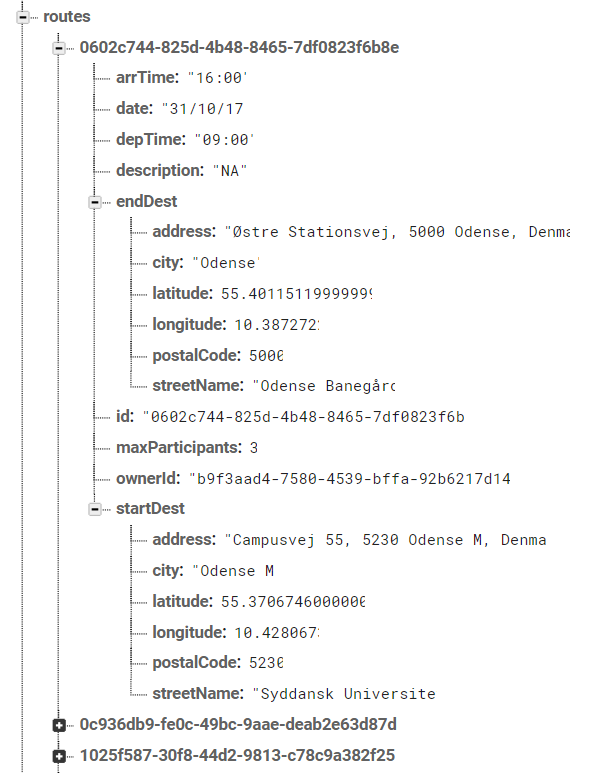
\includegraphics[scale=0.8]{Graphics/Images/firebase_routes.PNG}
        \caption{Route objects in Firebase}
        \label{fig:firebase_routes}
    \end{minipage}%
    \begin{minipage}{0.5\textwidth}
        \centering
        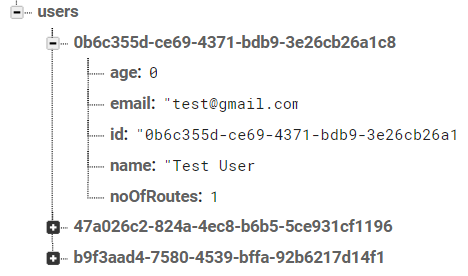
\includegraphics[scale=0.8]{Graphics/Images/firebase_users.PNG}
        \caption{User objects in Firebase}
        \label{fig:firebase_users}
    \end{minipage}
\end{figure}

Each route has a GUID key which can be referenced from other objects. For instance does each route contain a user reference as "ownerId". The "startDest" and "endDest" values could also be created as references to a new GeoPosition object in Firebase to reduce tree depth and avoid redundant data.
Connecting participants to a route is not implemented yet, but it would have been done as a "participant" list of user references for each route to maintain the flat tree structure. Changes in these objects has to be reflected in the domain classes, because the data snapshot automatically serializes the objects to a defined class structure. Therefore the data structure is a trade-off between best-practices of the firebase structure and the domain class structures.

The data retrieval is implemented in the "FirebaseDbHelper" class which implements a defined "IStorage" interface using the listeners "OnGetRoutesListener" and "OnGetUsersListener" due to asynchronous data retrieval. This structure is setup as modular as possible to ensure the database easily can be replaced with different technologies or database types. 

\subsection{Design}
The "BikeBus" application follows the "Material Design" principles created by Google\footnote{\url{https://material.io/guidelines/#}}, which are quite popular for Android apps. Material Design has great guidelines on how to improve mobile user experience and can quickly make the application look more professional.

The Android GUI components used to provide the Material Design elements:
\begin{itemize}
    \item CardView - The card element containing information of the bikebus
    \item RecyclerView - Infinity scroll view containing only cardviews
    \item BottomNavigationView - The bottom navigation menu between search, routes and profile tabs
    \item TabLayout with ViewPager - A Tab view in the profile view which switches between the profile and statistics fragment
    \item FloatingActionButton - The red create button
\end{itemize}

In this project Google API's has been frequently used for especially sensor data, but the Google AutoComplete

\begin{figure}[!htb]
\centering
\begin{minipage}{0.32\textwidth}
\centering
    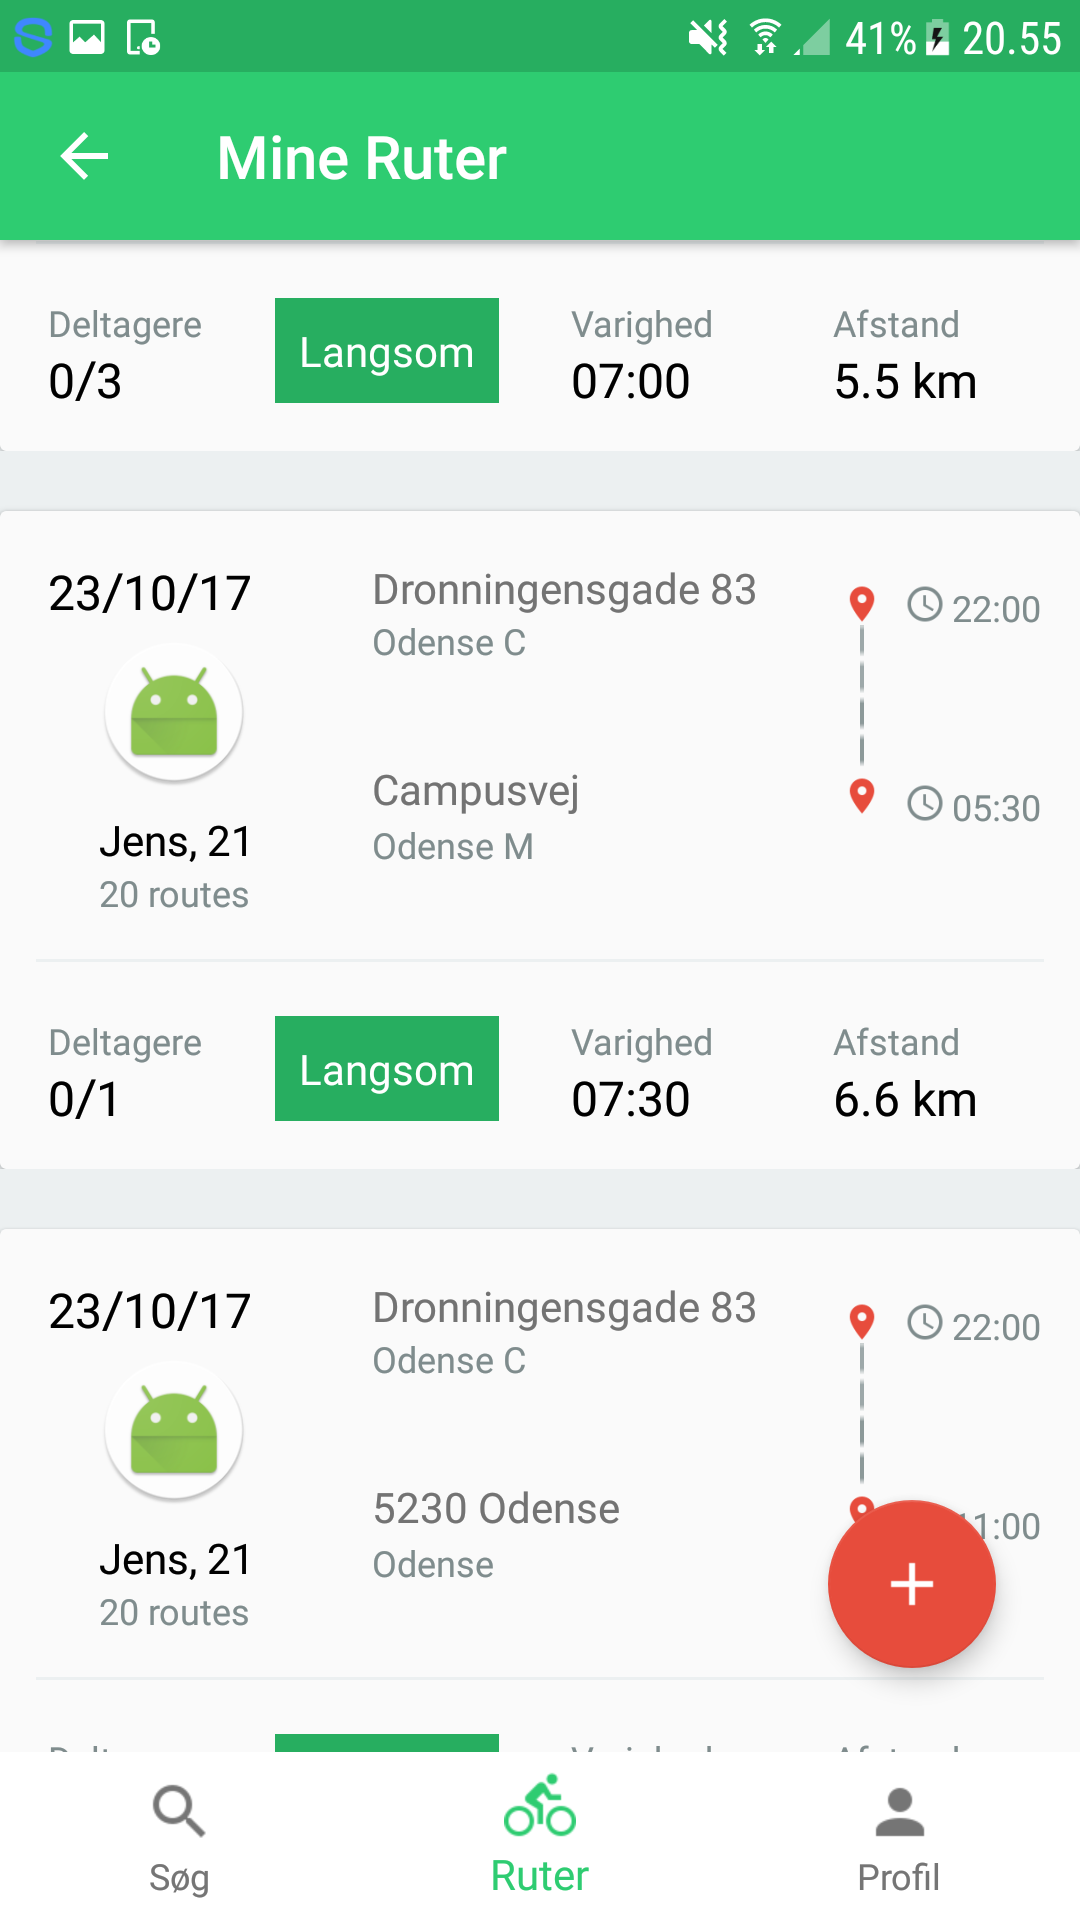
\includegraphics[width=\linewidth]{Graphics/Images/bikebus_search.png}
    \caption{Result page for BikeBus}
    \label{fig:sample_figure}
\end{minipage}\hfill
\begin{minipage}{0.32\textwidth}
\centering
    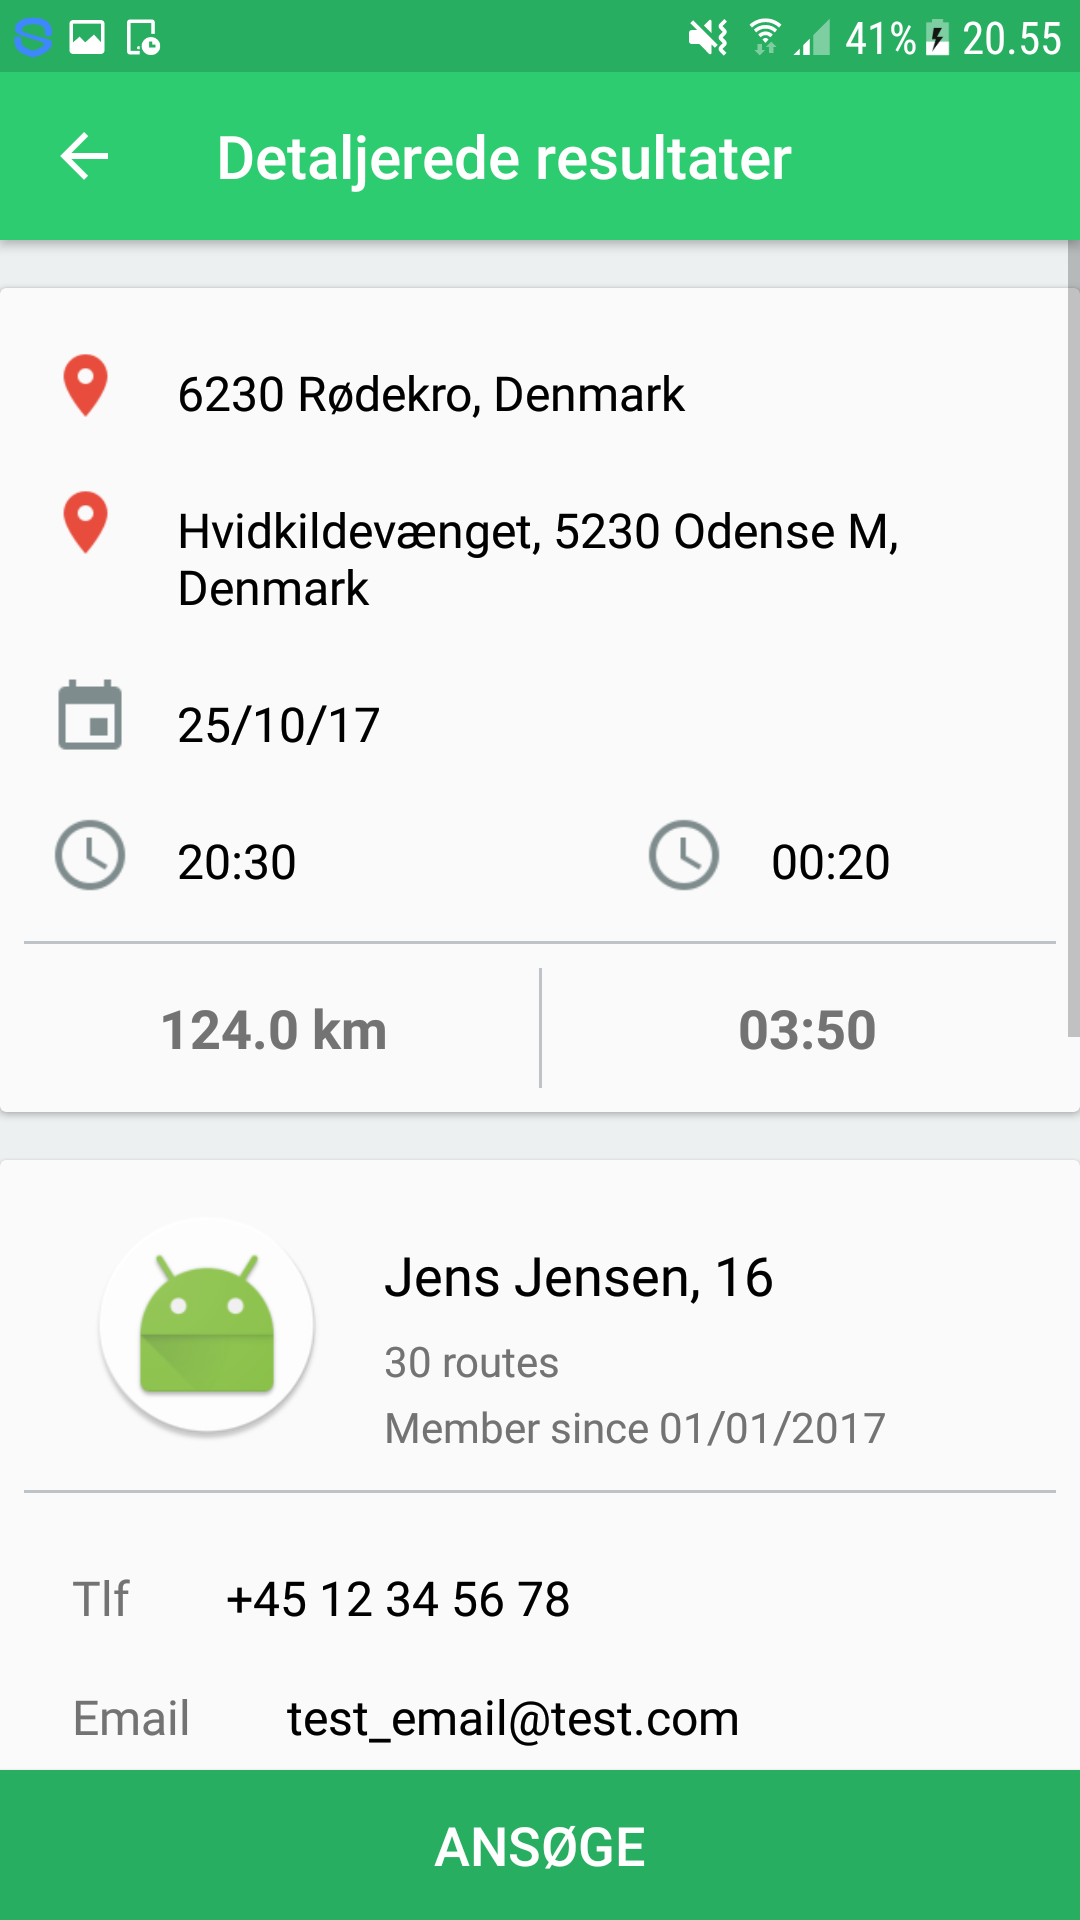
\includegraphics[width=\linewidth]{Graphics/Images/bikebus_detail_1.png}
    \caption{Detailed page for BikeBus (part 1)}
    \label{fig:sample_figure}
\end{minipage}\hfill
\begin{minipage}{0.32\textwidth}
\centering
    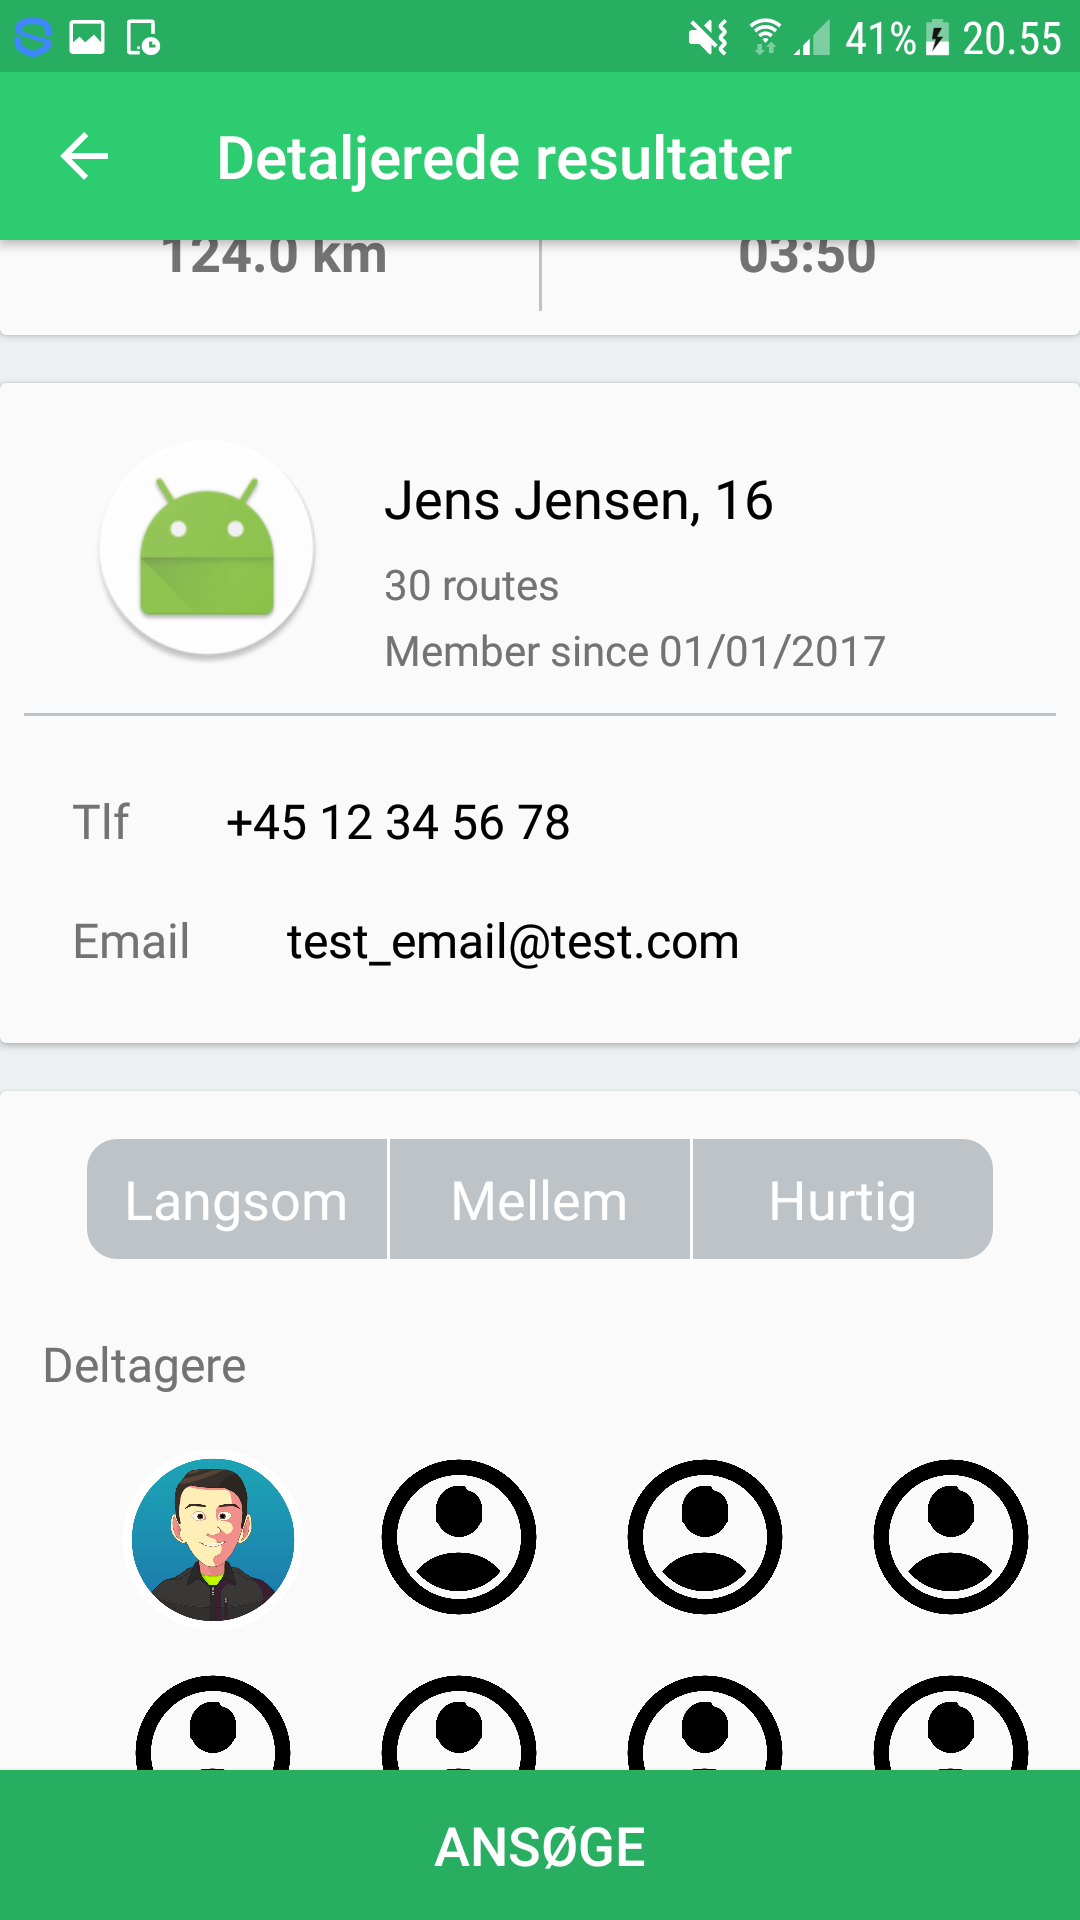
\includegraphics[width=\linewidth]{Graphics/Images/bikebus_detail_2.png}
    \caption{Detailed page for BikeBus (part 2)}
    \label{fig:sample_figure}
\end{minipage}
\end{figure}